\chapter{Fundamentação Teórica}
\begin{flushright}
	\begin{minipage}{14.0cm}
			\setlength{\parindent}{0cm}
			\textit{Neste capítulo é apresentada uma breve explanação sobre ..... Na Seção \ref{sec:fund_introdutoria} é apresentado um resumo sobre ..... Na Seção \ref{sec:fund_mais_uma} é descrito ..... Na Seção \ref{sec:fund_sobre_algo} é feita uma comparação .... A Seção \ref{sec:fund_resumo_cap} é um resumo do capítulo. \textbf{(item opcional)}}
	\end{minipage}
\end{flushright}


\section{Seção introdutória}\label{sec:fund_introdutoria}
\lipsum[1]
\section{Mais uma Seção}\label{sec:fund_mais_uma}
A fonte de todos os parágrafos de texto devem ser Times 12, com espaçamento 1,5 e recuo de primeira linha em 1,5. A Figura \ref{fig:grafico_excel} apresenta um gráfico do Excel exportado em PDF, dessa forma a imagem fica vetorial ao invés de rasterizada. Dessa forma você pode aumentar o zoom que os pixels da imagem nunca não irão estourar.

\begin{figure}[htb]
	\centering
	\setlength{\captionmargin}{-40pt}
	\caption{Gráfico produzido em Excel e salvo como PDF}\label{fig:grafico_excel}
    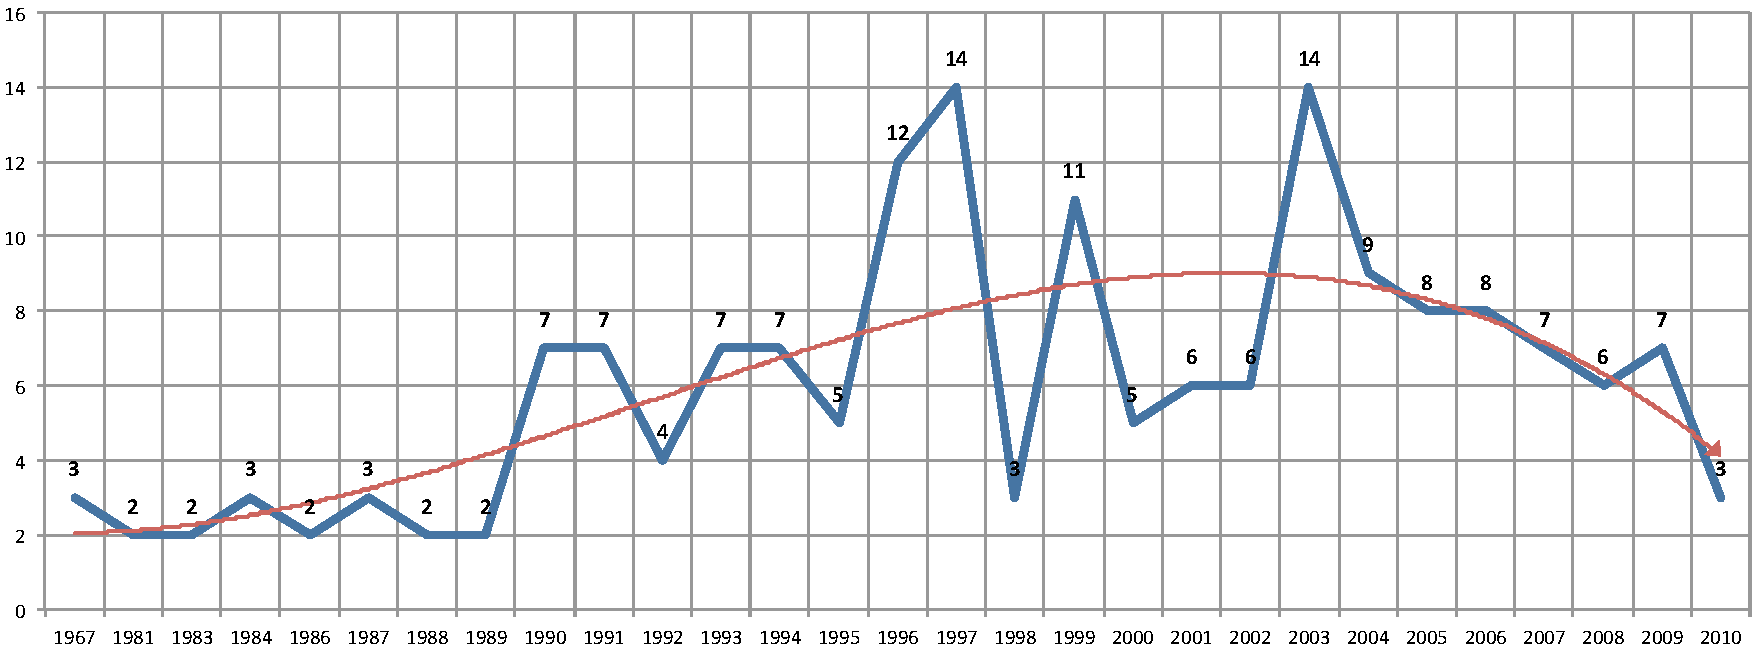
\includegraphics[scale=0.5]{imagens/abntex2-modelo-img-grafico.pdf}
	\legend{\textmd{Fonte: \citeonline[p. 24]{araujo2012}}}
\end{figure}

Todas as figuras ou tabelas inseridas no trabalho, deve ser comentada no texto, e devem ser chamadas pela sua numeração dentro do texto, e não como ``a figura abaixo ou acima''. As figuras e tabela devem ser centralizada com legenda no formato ``Figura x – texto'' ou ``Tabela x – texto'' vindo antes da mesma usando Times 10, negrito, espaçamento 1,5 e centralizada e após a figura ou tabela referenciar a fonte. Segundo a \cite{NBR14724:2011} ``...após a ilustração, na parte inferior, indicar a fonte consultada (elemento obrigatório, mesmo que seja produção do próprio autor), legenda, notas e outras informações necessárias à sua compreensão (se houver). A ilustração deve ser citada no texto e inserida o mais próximo possível do trecho a que se refere.''
\section{Seção que fala sobre algo}\label{sec:fund_sobre_algo}
Escrever algo para referenciar a Tabela \ref{tab:anova_delineamento}.
\begin{table}[htb]
\tiny
\caption{ANOVA pra delineamento em quadrado latino}
\label{tab:anova_delineamento}
\centering
\begin{tabular}{ll p{4.5cm} ll}
    \specialrule{.1em}{.05em}{.05em}
    \textbf{Fontes} & \textbf{g.1}  & \textbf{SQ}  & \textbf{E(SQ)} & F0 \\
    \specialrule{.1em}{.05em}{.05em}
    Tratamento & $(t-1)$  & $SQTratamento = \frac{1}{t}\displaystyle\sum_{j=1}^{t} y_j^2 - \frac{y^{2}}{N}$ &  $\frac{SQ_{Tratamento}}{t-1}$ & $\frac{E(SQ)_{Tratamento}}{E(SQ)_{erro}}$ \\
    %\hline
    Linha & $(t-1)$ & $SQLinha = \frac{1}{t}\displaystyle\sum_{i=1}^{t} y_i^2 - \frac{y^{2}}{N}$  & $\frac{SQ_{Linha}}{t-1}$ & \\
    %\hline
    Coluna & $(t-1)$ & $SQColuna = \frac{1}{t}\displaystyle\sum_{k=1}^{t} y_k^2 - \frac{y^{2}}{N}$ & $\frac{SQ_{Coluna}}{t-1}$ &  \\
    %\hline
    Erro & $(t-1) (t-2)$ & $SQ_{Erro} = SQ_{Total} - SQ_{Linha} - SQ_{Tratamento} - SQ_{Coluna}$ & $\frac{SQ_{Erro}}{(t-2)(t-1)}$ &  \\
    \specialrule{.1em}{.05em}{.05em}
    Total & $t^{2}-1$ & $\displaystyle\sum_{i}\sum_{j}\sum_{k} y_{ijk}^2 - \frac{y^{2}}{N}$ &  &  \\
    %\hline
	
\end{tabular}
\\[8pt]
\fbox{\begin{minipage}{1.5cm}
\textbf{Legenda:}\\
\end{minipage}
\begin{minipage}{12cm}
$g.1 \rightarrow$ Grau de liberdade; $SQ \rightarrow$ Soma dos quadrados; $E(SQ) \rightarrow$ Valor esperado dos quadrados médio; $F_{0} \rightarrow$ Estatística de teste $F$
\end{minipage}
}
\legend{\textmd{Fonte: \citeonline{demery2012}}}
\end{table}

Quando a figura, quadro ou tabela pertencerem ao próprio autor referenciar a fonte como ``Elaborada pelo autor''. Pode-se visualizar essa autorreferência no Quadro \ref{quadro:exemplo}.

\begin{quadro}[htb]
\caption{Exemplo de quadro}\label{quadro:exemplo}
\centering
\begin{tabular}{ccc}
    \specialrule{.1em}{.05em}{.05em}
    \textbf{Situação} & \textbf{mmol/L}  & \textbf{mg/dL} \\
    \hline
    Em jejum e antes das refeições & 7,0 & 126 \\
    Uma hora depois de uma refeição & 10,0 & 180 \\
    Duas horas depois de uma refeição & 8,0 & 144 \\
    Antes de dormir (mínimo) & 6,0 & 108 \\
    \specialrule{.1em}{.05em}{.05em}
\end{tabular}
\legend{\textmd{Fonte: Elaborado pelo autor}}
\end{quadro}


\section{Resumo do capítulo}\label{sec:fund_resumo_cap}
Escrever o resumo do capítulo. Esta seção é obrigatória, porém o título poderá ser modificado como exemplo: considerações finais do capítulo, conclusão do capítulo, etc…

